\begin{enumerate}
	\item L'utilisateur se rend sur la page de connection en cliquant sur \textit{Login}
	\item Il entre son nom d'utilisateur et son mot de passe.
	\item Après vérification, l'utilisateur est redirigé vers la page d'accueil. 
\end{enumerate}

\begin{figure*}[h!]
	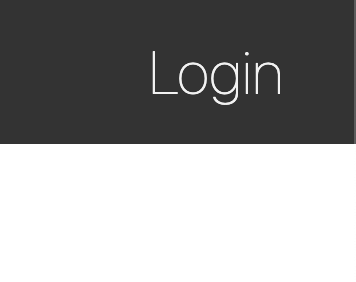
\includegraphics[width = 0.5\textwidth,center]{Figures/us0-1}
	\caption{Bouton de connection}
\end{figure*}

\newpage
\begin{figure*}[h!]
	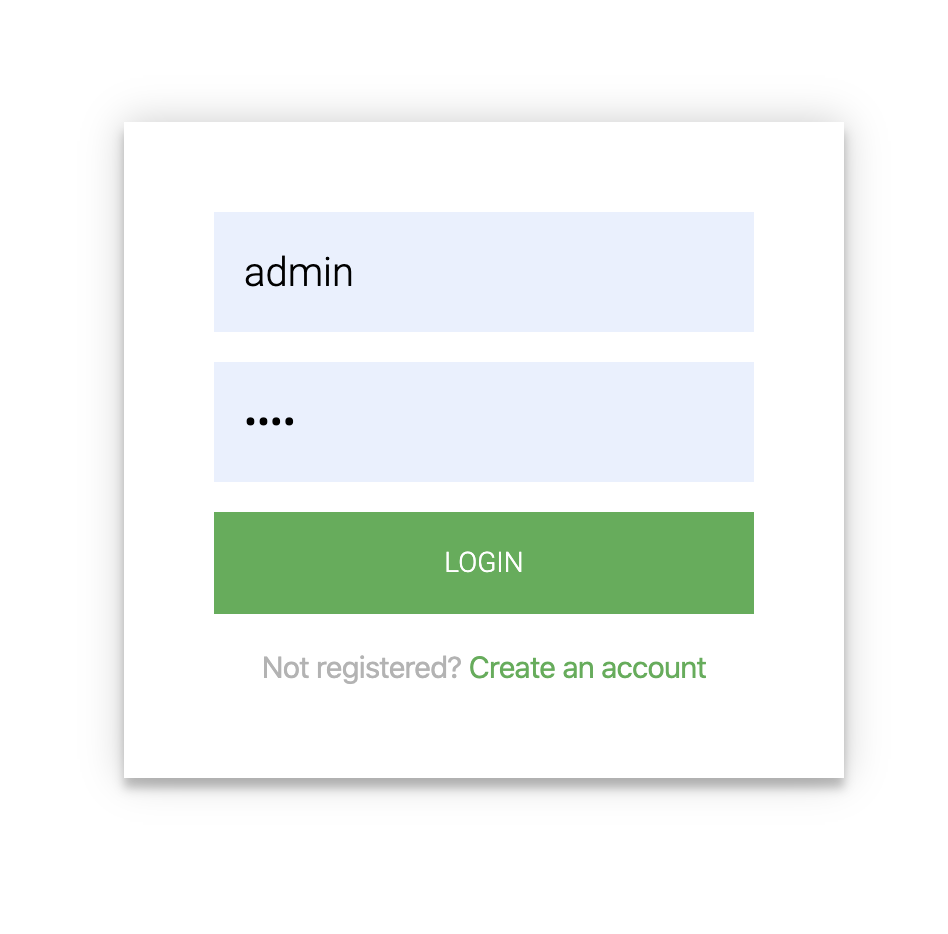
\includegraphics[width = 0.5\textwidth,center]{Figures/us0-2}
	\caption{Formulaire de connection}
\end{figure*}

\subsubsection{Gestion des erreurs et des risques}
	\paragraph{}
		En cas d'erreur dans les informations de connection fournis par l'utilisateur, une erreur sera produite et affiché sur le site.

\newpage
\subsubsection{Diagramme de séquence}
	\begin{figure*}[h!]
		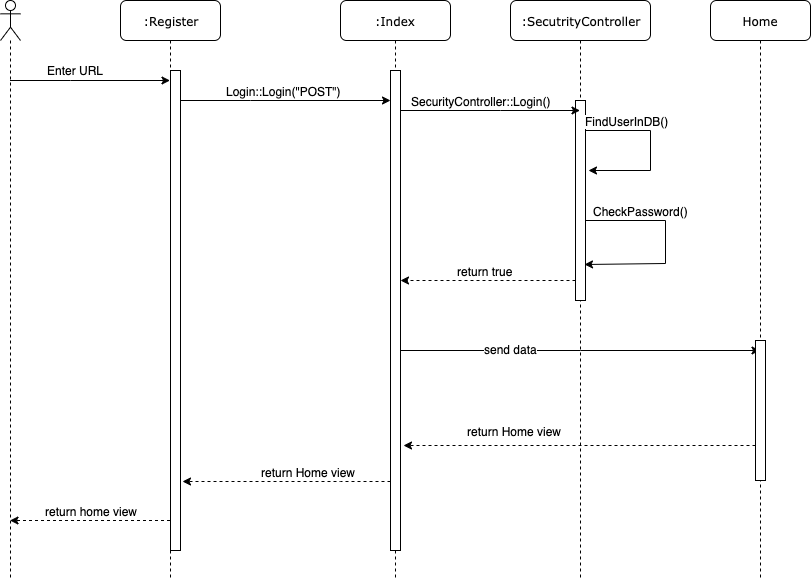
\includegraphics[width = \textwidth,center]{Diagramme/sequence-us0}
		\caption{Diagramme de séquence de la connections d'un utilisateur}
	\end{figure*}

\subsubsection{Scripts concernés}
	\begin{itemize}
		\item \Href{https://github.com/victorsmits/Aquabike/blob/master/Symfony-Twig/templates/security/login.html.twig}{login.html.twig}
		\item \Href{https://github.com/victorsmits/Aquabike/blob/master/Symfony-Twig/src/Entity/Person.php}{Person.php}
		\item \Href{https://github.com/victorsmits/Aquabike/blob/master/Symfony-Twig/src/Controller/SecurityController.php}{SecurityController.php}
	\end{itemize}